\section{Introduction}
\label{sec:intro}

Gammapy is a Python package for gamma-ray astronomy.

\subsection{Things we could mention}

Here's a list of references I'd like to cite ... to be incorporated into the
main text somewhere:

\begin{itemize}
\item The Python programming language\footnote{\PythonUrl}
\item Gammapy webpage\footnote{\GammapyUrl}
\item Astropy \citep{astropy}
\item PyFACT \citep{pyfact}
\item FITS \citep{fits}
\item Gamma-astro data formats \cite{gadf-zenodo}
\item Sherpa \citep{sherpa-2011, sherpa-2009}
\item Naima\footnote{\NaimaUrl} \citep{Naima}
\item Gammapy use in science publications: \citep{Owen2015}, SNR shell, HGPS
\end{itemize}


\begin{figure}[t]
\centering
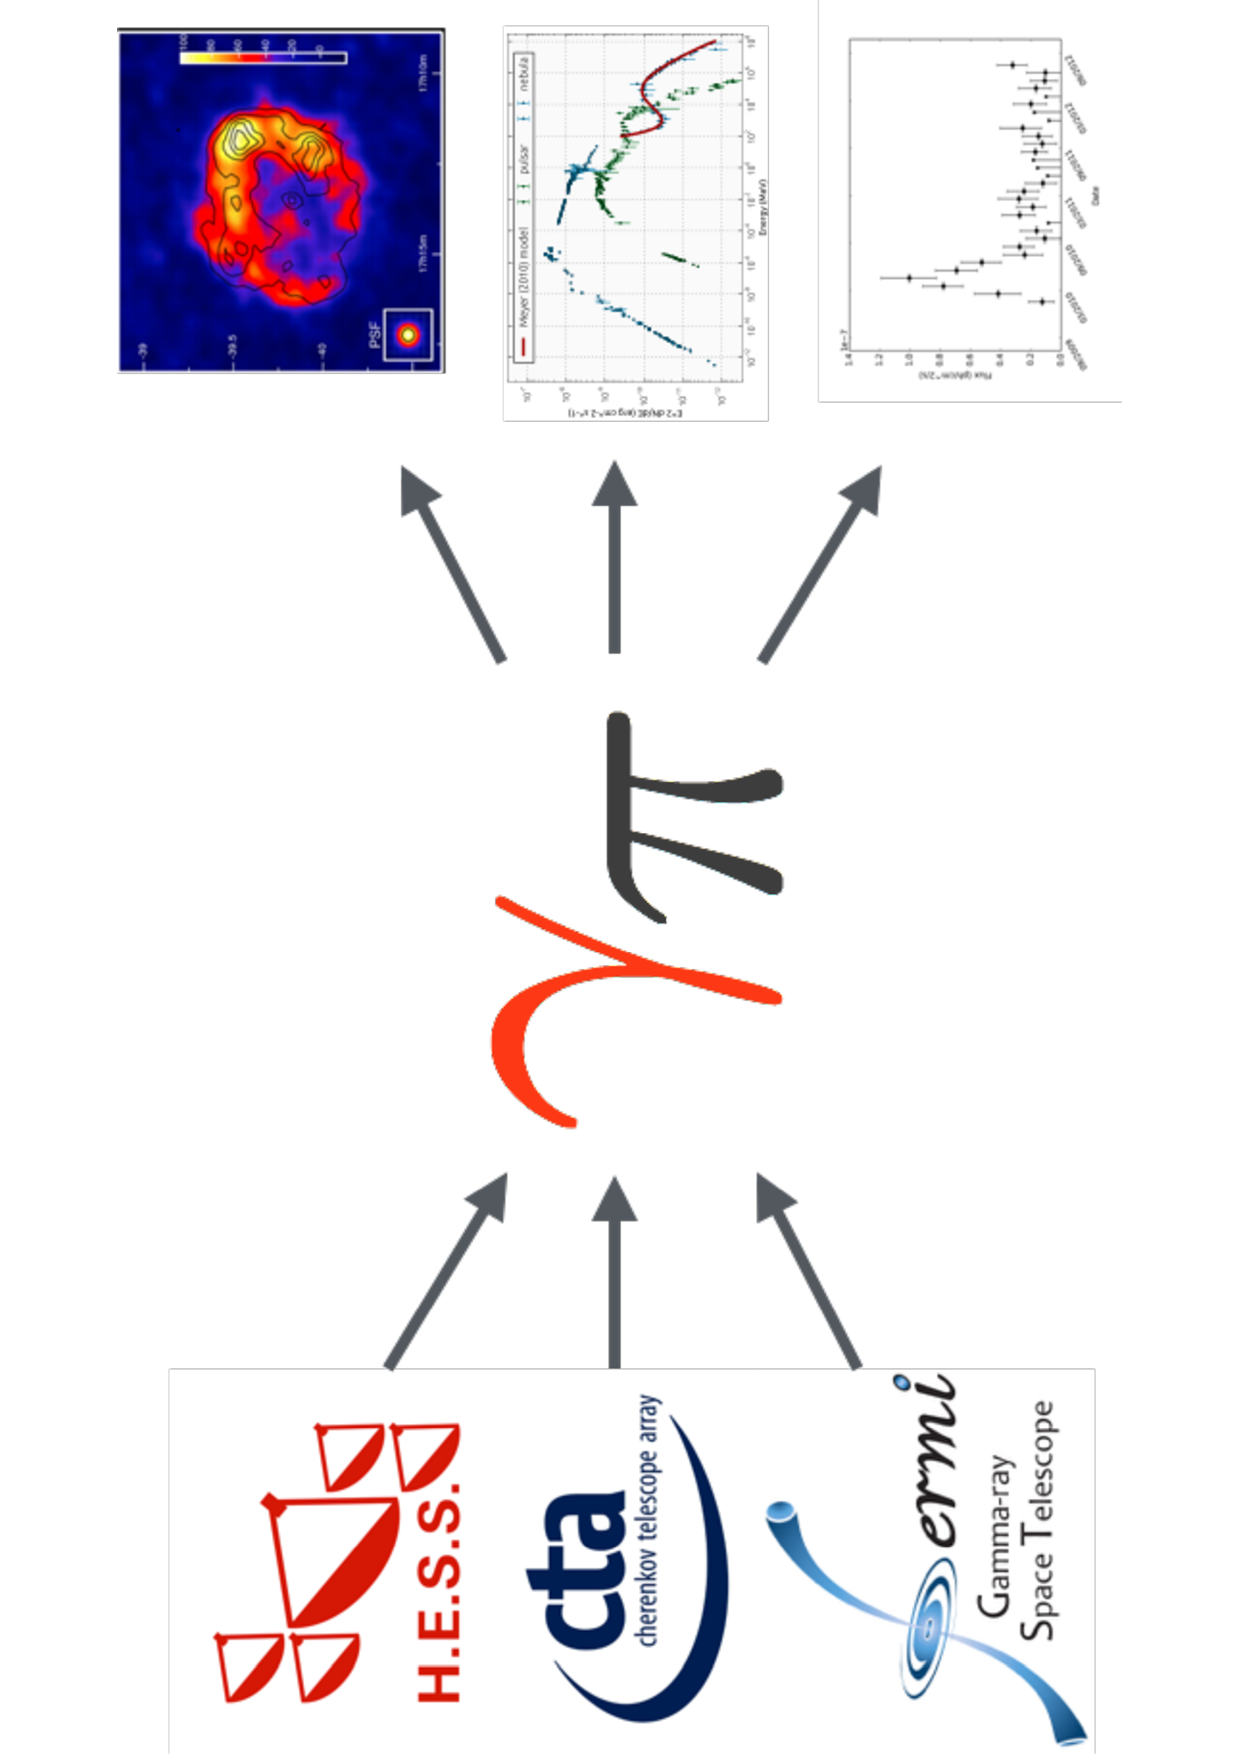
\includegraphics[height=0.5\textwidth, angle=270]{figures/gammapy-big-picture}
\caption{
Gammapy is a Python package for high-level gamma-ray data analysis. Using event
lists, exposures and point spread functions as input you can use it to generate
science results such as images, spectra, light curves or source catalogs. So far
it has been used to simulate and analyse H.E.S.S., CTA and \textit{Fermi}-LAT
data, hopefully it will also be applied to e.g. VERITAS, MAGIC or HAWC data in
the future.
}
\label{fig:big-picture}
\end{figure}

\begin{figure}[t]
\centering
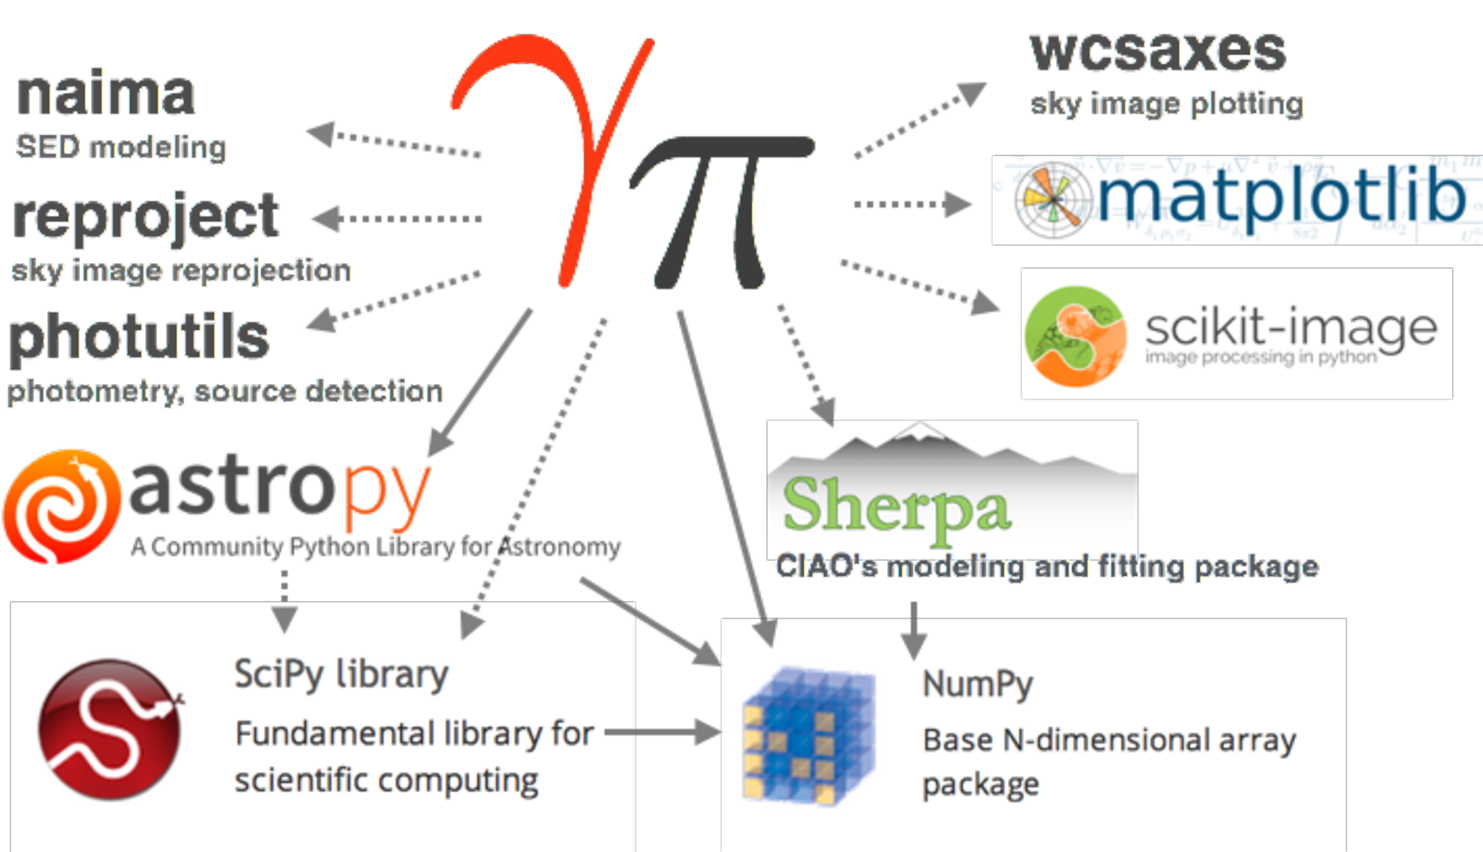
\includegraphics[width=0.5\textwidth]{figures/gammapy-dependencies}
\caption{
The Gammapy stack. Required dependencies Numpy and Astropy are illustrated with
solid arrows, optional dependencies (the rest) with dashed arrows.
}
\label{fig:dependencies}
\end{figure}
